%%%%%%%%%%%%%%%%%%%%%%%%%%%%%%%%%%%%%%%%%%%%%%%%%%%%%%%%%%%%%%%%%%
%%%%%%%% ICML 2014 EXAMPLE LATEX SUBMISSION FILE %%%%%%%%%%%%%%%%%
%%%%%%%%%%%%%%%%%%%%%%%%%%%%%%%%%%%%%%%%%%%%%%%%%%%%%%%%%%%%%%%%%%

% Use the following line _only_ if you're still using LaTeX 2.09.
%\documentstyle[icml2014,epsf,natbib]{article}
% If you rely on Latex2e packages, like most moden people use this:
\documentclass{article}

% use Times
\usepackage{times}
% For figures
\usepackage{graphicx} % more modern
%\usepackage{epsfig} % less modern
\usepackage{subfigure} 

\usepackage{verbatim}

% For citations
\usepackage{natbib}

% For algorithms
\usepackage{algorithm}
\usepackage{algorithmic}

% As of 2011, we use the hyperref package to produce hyperlinks in the
% resulting PDF.  If this breaks your system, please commend out the
% following usepackage line and replace \usepackage{icml2014} with
% \usepackage[nohyperref]{icml2014} above.
\usepackage{hyperref}

% Packages hyperref and algorithmic misbehave sometimes.  We can fix
% this with the following command.
\newcommand{\theHalgorithm}{\arabic{algorithm}}

% Employ the following version of the ``usepackage'' statement for
% submitting the draft version of the paper for review.  This will set
% the note in the first column to ``Under review.  Do not distribute.''
\usepackage[accepted]{icml2014} 


% The \icmltitle you define below is probably too long as a header.
% Therefore, a short form for the running title is supplied here:
\icmltitlerunning{Jing, Xu, Tian, Huang}

\begin{document} 

\twocolumn[
\icmltitle{Stock price prediction with LSTM network\\Project Progress Report for COMP 562}

% It is OKAY to include author information, even for blind
% submissions: the style file will automatically remove it for you
% unless you've provided the [accepted] option to the icml2014
% package.
\icmlauthor{Siyang Jing}{siyangj@live.unc.edu}
\icmlauthor{Jiyu Xu}{xujiyu@live.unc.edu}
\icmlauthor{Jiacheng Tian}{jctian@live.unc.edu}
\icmlauthor{Yuhui Huang}{yuhui97@live.unc.edu}

% You may provide any keywords that you 
% find helpful for describing your paper; these are used to populate 
% the "keywords" metadata in the PDF but will not be shown in the document
\icmlkeywords{boring formatting information, machine learning}

\vskip 0.3in
]

\begin{abstract} 
The time series of stock prices are non-stationary and nonlinear, making the prediction of future price trends much challenging. To learn long-term dependencies of stock prices, we first perform unsupervised learning to extract and construct useful features, then build a deep Long Short-Term Memory (LSTM) network to generate the prediction. The experiments on real market dataset demonstrate that the proposed model outperforms other four baseline models in the mean square error.
\end{abstract} 

\section{Introduction}

In the financial industry, stock price prediction has constantly been a popular field of research. According to many widely accepted studies, stock markets have been proved to be predictable in some scenarios. While different features are available for prediction, it's interesting to focus solely on past trading patterns. In the last decade, there has been a huge increase in the application of deep neural network. As a result, applying deep learning on stock market prediction has become a field of interest.

\subsection{Literature Review}

Our research assumes minute-level price fluctuation pattern is independent of corporate fundamentals and macro economy. Thus, unlike the studies of \cite{Chiang2016}, \cite{Chourmouziadis2016}, and \cite{Zhong2017} in which daily price data are used as input, we seek to develop a predictive model based on minute-level price data. The prediction of future stock price had also been understood as both classification and regression problems in previous studies. \cite{Chen2016} and \cite{Zhong2017} provided prediction of market direction as either up or down. In more complicated cases, \cite{Chourmouziadis2016} specified cash and stock within the optimal portfolio composition. Our study intends to give a prediction of the stock return of the next minute.

There have been linear and nonlinear models to predict stock price movement with varying degrees of success. \cite{Chong2017} noted a multilayer artificial neural network might be particularly suitable with such time-series data, due to its higher computational power and sophistication of algorithm. Such model selects features based on raw input price data automatically and does not require understanding or providing data from the side of fundamentals or macro economy, which fits our assumption about minute-level price fluctuation pattern. For performance measurement, previous studies have used trade simulation or various MSE methods \cite{Chiang2016}; \cite{Chourmouziadis2016}; \cite{Zhong2017}; \cite{Chong2017}.

\subsection{Data}

Due to certain limitation and just for preliminary testing of our strategy, we are currently using 10 days of minute-level price data of 50 stocks, in total of 3900 time steps. Our aim is to obtain data of 10 years for model training. Each stock, at each time step, has 5 features, open/high/low/close price and volume. Therefore, in total, each time step contains 250 features. The input will contain 60 lagged time step, and we aim to predict the close prices of the 50 stocks at next time step. We may adjust the number of lagged periods for better performance later. We use the first 9 days as training, and the last day as test.

\section{Method}
Our model will be composed of two parts, with the first part being unsupervised learning with traditional ML techniques like RBM, PCA, etc. The second part takes advantage of recurrent neural network (RNN) model, especially its variant LSTM. 

\subsection{Model}

Following the practice in the research of Chong et al.\cite{Chong2017}, our model takes the form of
\[r_{t+1}=f\circ\phi(R_t)+\gamma,\,\gamma\sim\mathcal{N}(0,\beta).\]
We assume the return of one hour prior to the current time point has influence on the return of the stock in the next minute, so $t$ is in unit of minutes. As mentioned above, $R_t$ is the $250\times 60$ dimensional raw level input vector. $\phi$ transforms the data to features, or representations. It hasn't been implemented. $f$ is the predictor function, and is learned using RNN, which seems to be the state of the art method \cite{Abe2018}. Specifically, we use a network with 10 layer, each with 1000 LSTM units.

\subsection{Loss Function and Training}
We can formulate the problem in two ways.
\begin{enumerate}
	\item Explicitly make the output dependent on the previous 60 time steps. We unroll the network for 60 time steps, and only calculate the MSE loss between the final output and the truth. This way, when we perform prediction, we should probably first run the model for 60 time steps and then only take the last output.
	\item Make the training sequence to sequence, unroll the network for arbitrary time steps, and optimize against the MSE loss between the output sequence and the truth sequence.
\end{enumerate}
 
\section{Preliminary Results} 
We first transform the price data to returns, i.e.
\[r_{t+1} = \frac{x_{t+1}-x_{t}}{x_{t}}.\]
We then normalize the volume data by
\[v_{n,t+1} = \frac{v_{n,t+1}-m_{n}}{\sigma_{n}},\]
where $m_n$ and $\sigma_n$ are the mean and standard deviation of the volumes of all time steps of stock $n$.

\subsection{Evaluation}
To evaluate our model performance on the test set, we employ the most popular and probably the standard validation strategy in time series analysis, the Walk Forward Validation strategy, where we do not retrain our model on each time step, but we make the last tested data point available to the model. In the case of our RNN, we do not reset the initial state, and simply let the model run forward to make prediction at each time step.

In terms of evaluation metrics, we use mean squared error (MSE), mean relative absolute error (RE), and trend error rate (TE), which is the rate of predicting the wrong trend (e.g. positive return predicted as negative return).

\subsection{Results}
We compare our method with two popular statistical methods ARIMA and GARCH, the method from \cite{Chong2017}, and a simple feed forward network of 10 layers, each with 250 neurons to make the total number parameters roughly equal to that of our LSTM network. Table-\ref{comparison-table} shows the results.

\begin{table}[t]
\caption{Comparison between different methods with various metrics.}
\label{comparison-table}
\vskip 0.15in
\begin{center}
\begin{small}
\begin{sc}
\begin{tabular}{lcccr}
\hline
\abovespace\belowspace
Method & MSE ($10^{-7}$) & RE (\%) & TE (\%) \\
\hline
\abovespace
Proposed   & 8.5& 9.5& 0.05  \\
arima      & 73.2& 25.8& 0.23 \\
garch      & 85.6& 38.1& 0.25  \\
Chong 2017 & 40.7& 19.7& 0.21     \\
\belowspace
Deep FNN   & 30.5& 17.5& 0.12 \\
\hline
\end{tabular}
\end{sc}
\end{small}
\end{center}
\vskip -0.1in
\end{table}

Figure-\ref{truth-pred-plot} plots the true price curve and the predicted price curve for 3 stocks.

\begin{figure}
  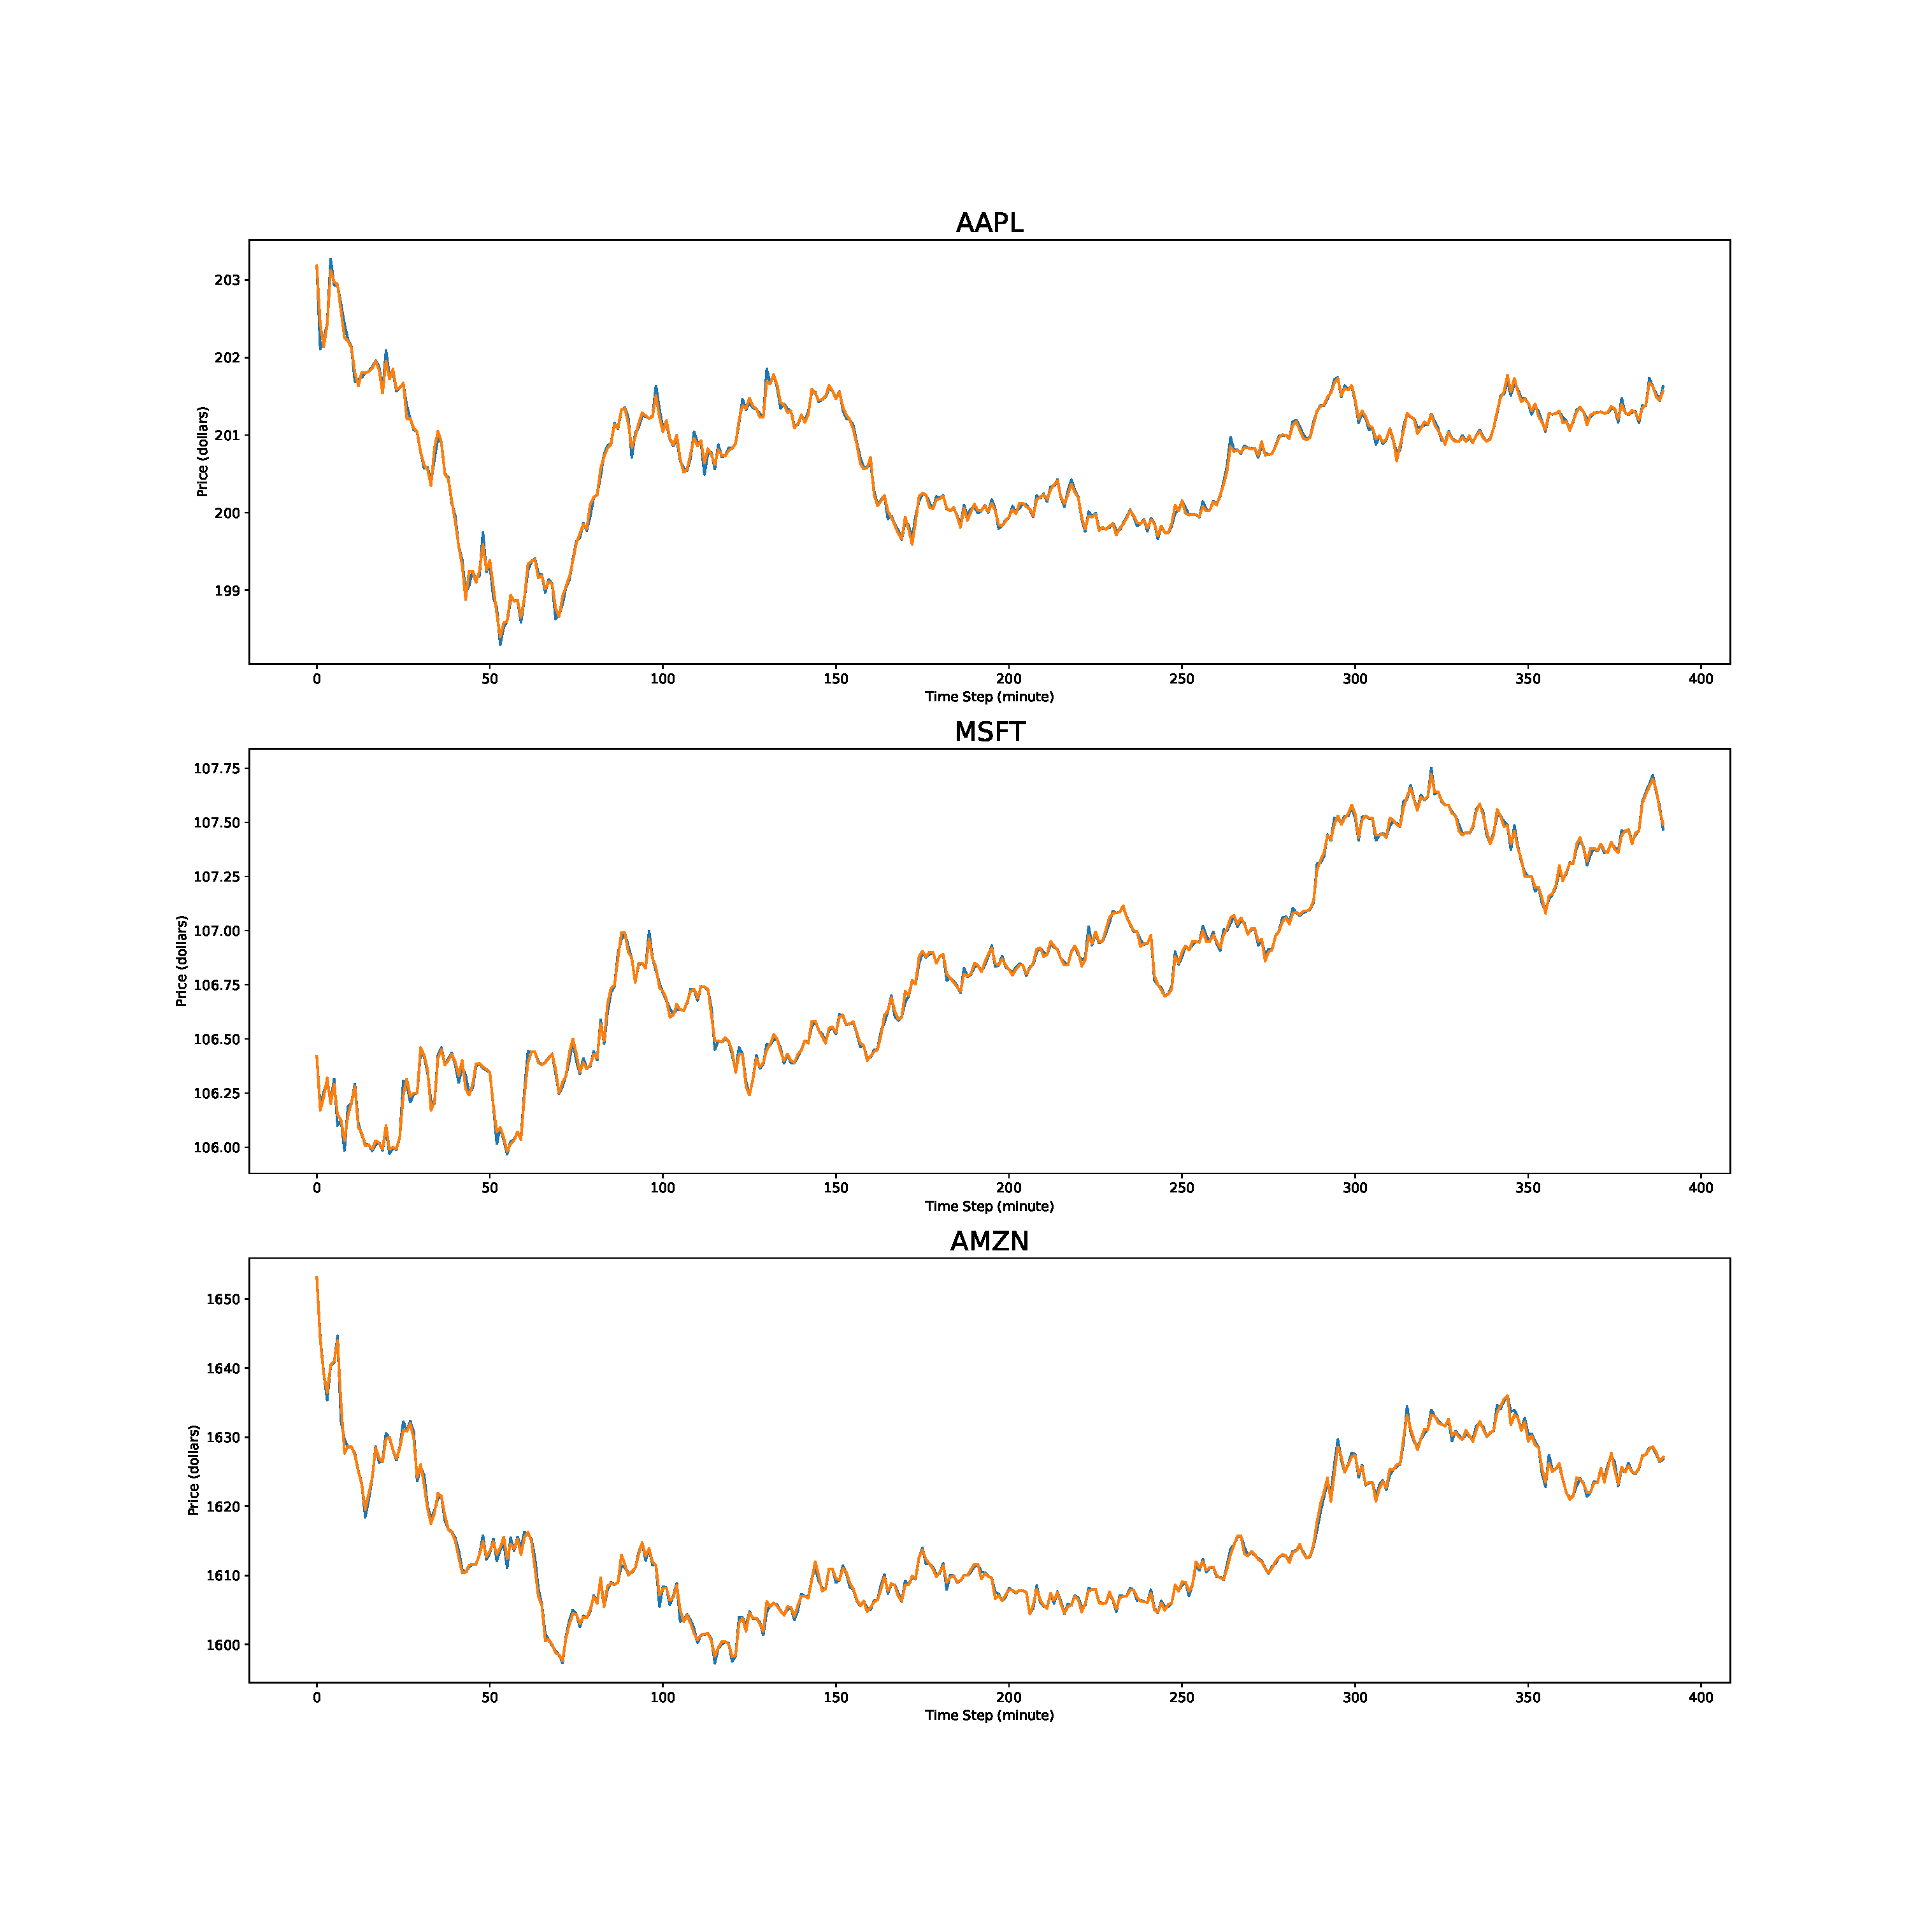
\includegraphics[width=\linewidth]{Figures/PredTruth_2.eps}
  \caption{Comparison between true and predicted price.}
  \label{truth-pred-plot}
\end{figure}

\section*{Acknowledgments} 
We thank Guoyan Zheng and Eason Chan for their LSTM and tensorflow code templates (not publicly available).

\bibliography{../Papers/Reference}
\bibliographystyle{icml2014}

\end{document} 